% Motivation paragraph
Theoretical motivation
in~\Cref{sec:hh_motivation}.\todo[inline]{Should say something that
  new physics could alter the self-coupling constant.}

In the current experimental environment of HEP, direct searches for
non-resonant Higgs boson pair production are the most sensitive probes
of the Higgs boson self-coupling constant, \lambdahhh, due to the
large sensitivity of the total and differential non-resonant \HH
production cross section to anomalous values of \lambdahhh. Hereafter,
the self-coupling constant is given in terms of the modifier
$\klambda = \lambdahhh / \lambdahhh^{\text{SM}}$ relating an assumed
value of the self-coupling constant to the value predicted by the SM.

The non-resonant \HH production cross section via \ggF and VBF is
shown in \Cref{fig:hh_xsec_incl} as a function of \klambda. The
production via \ggF is the dominant contribution to the total
non-resonant \HH production cross section throughout the considered
\klambda range.
% exceeding cross section of the VBF production mode by at elast a
% factor of about five (18 for SM \HH production).
For the \ggF production mode, the destructive interference between the
box and triangle diagram becomes maximal at about $\klambda = 2.3$ at
which point the cross section reaches a minimum of approximately
\SI{13}{\femto\barn}. Similar behaviour is shown for the VBF
production mode, although involving different diagrams (cf.\
\Cref{fig:hh_feynmans}) and yielding a minimum in cross section below
$\klambda = 2$.

\begin{figure}[htbp]
  \centering

  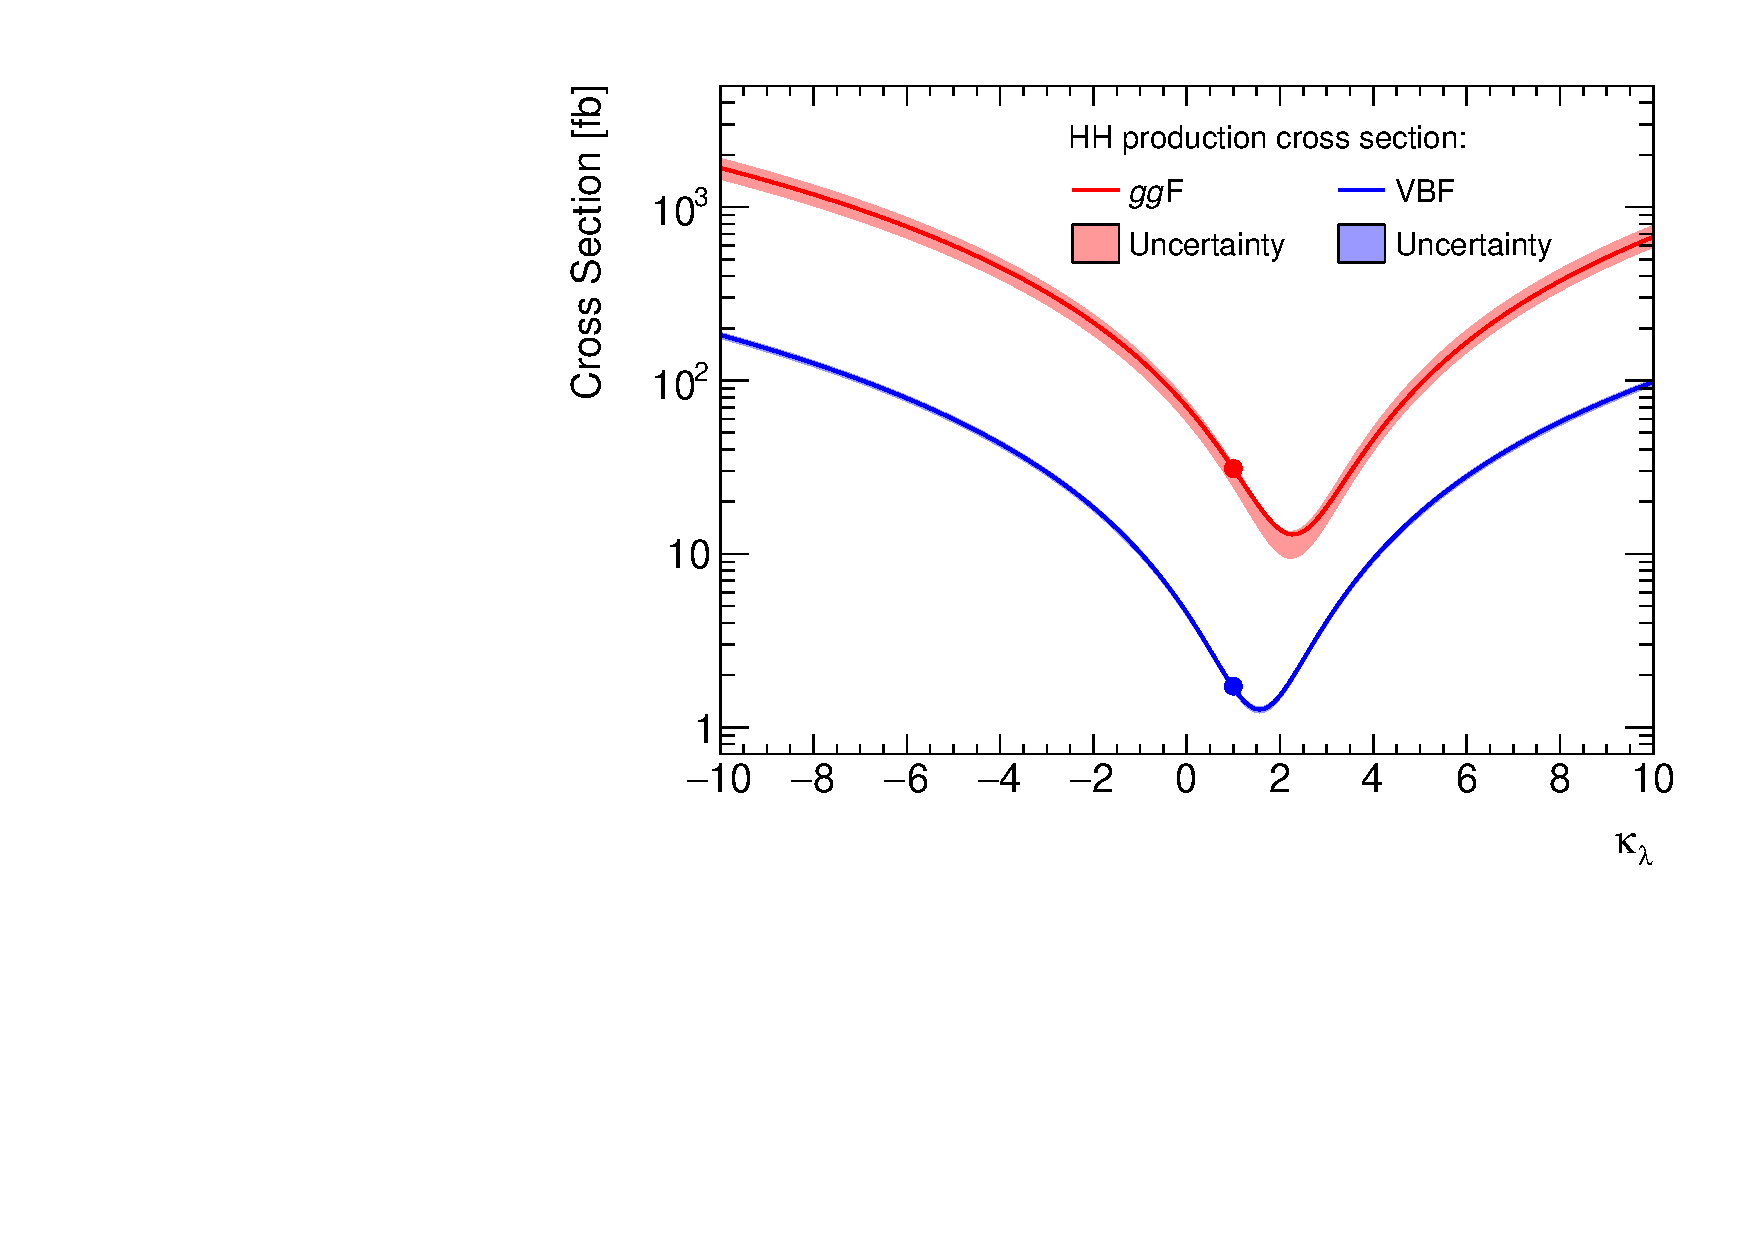
\includegraphics[width=0.55\textwidth]{self_coupling/hh_xsec}

  \caption{\HH production cross section via \ggF and VBF as a function
    of \klambda for $\mH = \SI{125.0}{\GeV}$ in \pp-collisions at
    $\sqrt{s} = \SI{13}{\GeV}$. The production cross section via \ggF
    is given at $\text{NNLO}_{\text{NLO-i}}$ rescaled to
    $\text{NNLO}_{\text{FTapprox}}$ in the $\klambda = 1$
    limit~\cite{Amoroso:2020lgh,Baglio:2020wgt,LHCHWGHH,Grazzini:2018bsd}. The
    production cross section via VBF is obtained from simulation with
    \MGNLO at LO after applying an $\text{N}^3\text{LO}$ $k$-factor
    derived for the SM case~\cite{Dreyer:2018qbw,LHCHWGHH}. The cross
    sections are parameterised as quadratic functions of
    \klambda. Theoretical uncertainties are shown as coloured bands.}%
  \label{fig:hh_xsec_incl}
\end{figure}

In addition to the change in total cross section, anomalous values of
\klambda alter the differential \HH production cross section primarily
in terms of the invariant mass of the pair of Higgs bosons. This is
shown in \Cref{fig:hh_xsec_mhh} for the dominant \ggF production mode
and for five exemplary values of \klambda. The \mHH spectra for
different values of \klambda show large differences in their
\emph{hardness} as measured by the median of the \mHH distribution
in~\Cref{fig:hh_median_mhh}. For \klambda values just below or at the
point of maximum destructive interference between the box and triangle
diagram, the \mHH spectra are moderately hard and have a pronounced
double peak structure. For other values of \klambda, particularly for
$\klambda \approx 3$, the cross section at low \mHH is enhanced
resulting in comparatively soft \mHH spectra.

\begin{figure}[htbp]
  \begin{subfigure}[t]{0.485\textwidth}
    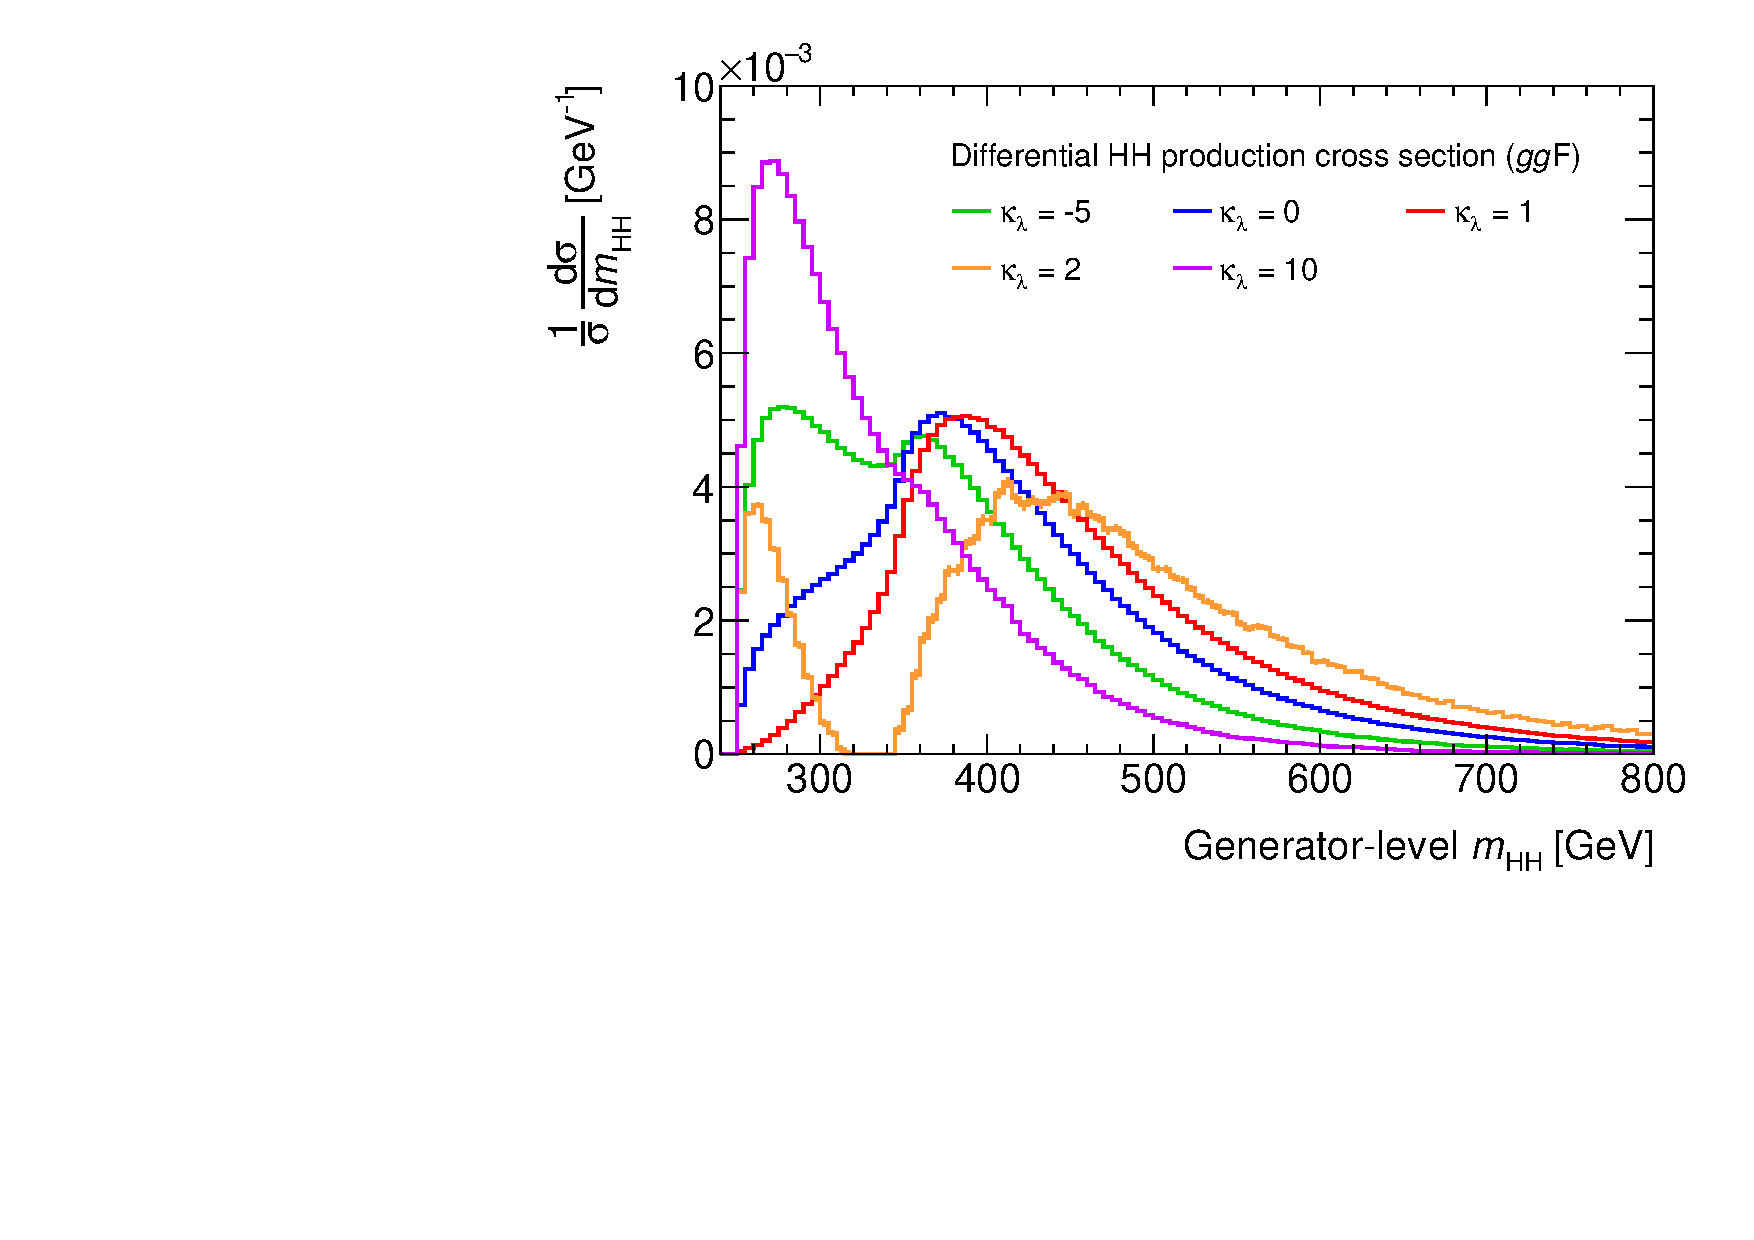
\includegraphics[width=\textwidth]{self_coupling/hh_mhh_vs_klam}
    \subcaption{Differential \HH production cross section with respect
      to \mHH for the \ggF production mode and selected values of
      \klambda. The differential cross sections are normalised by
      dividing by the total cross section. Only statistical
      uncertainties from the finite number of generated events are
      shown.}%
    \label{fig:hh_xsec_mhh}
  \end{subfigure}\hfill%
  \begin{subfigure}[t]{0.485\textwidth}
    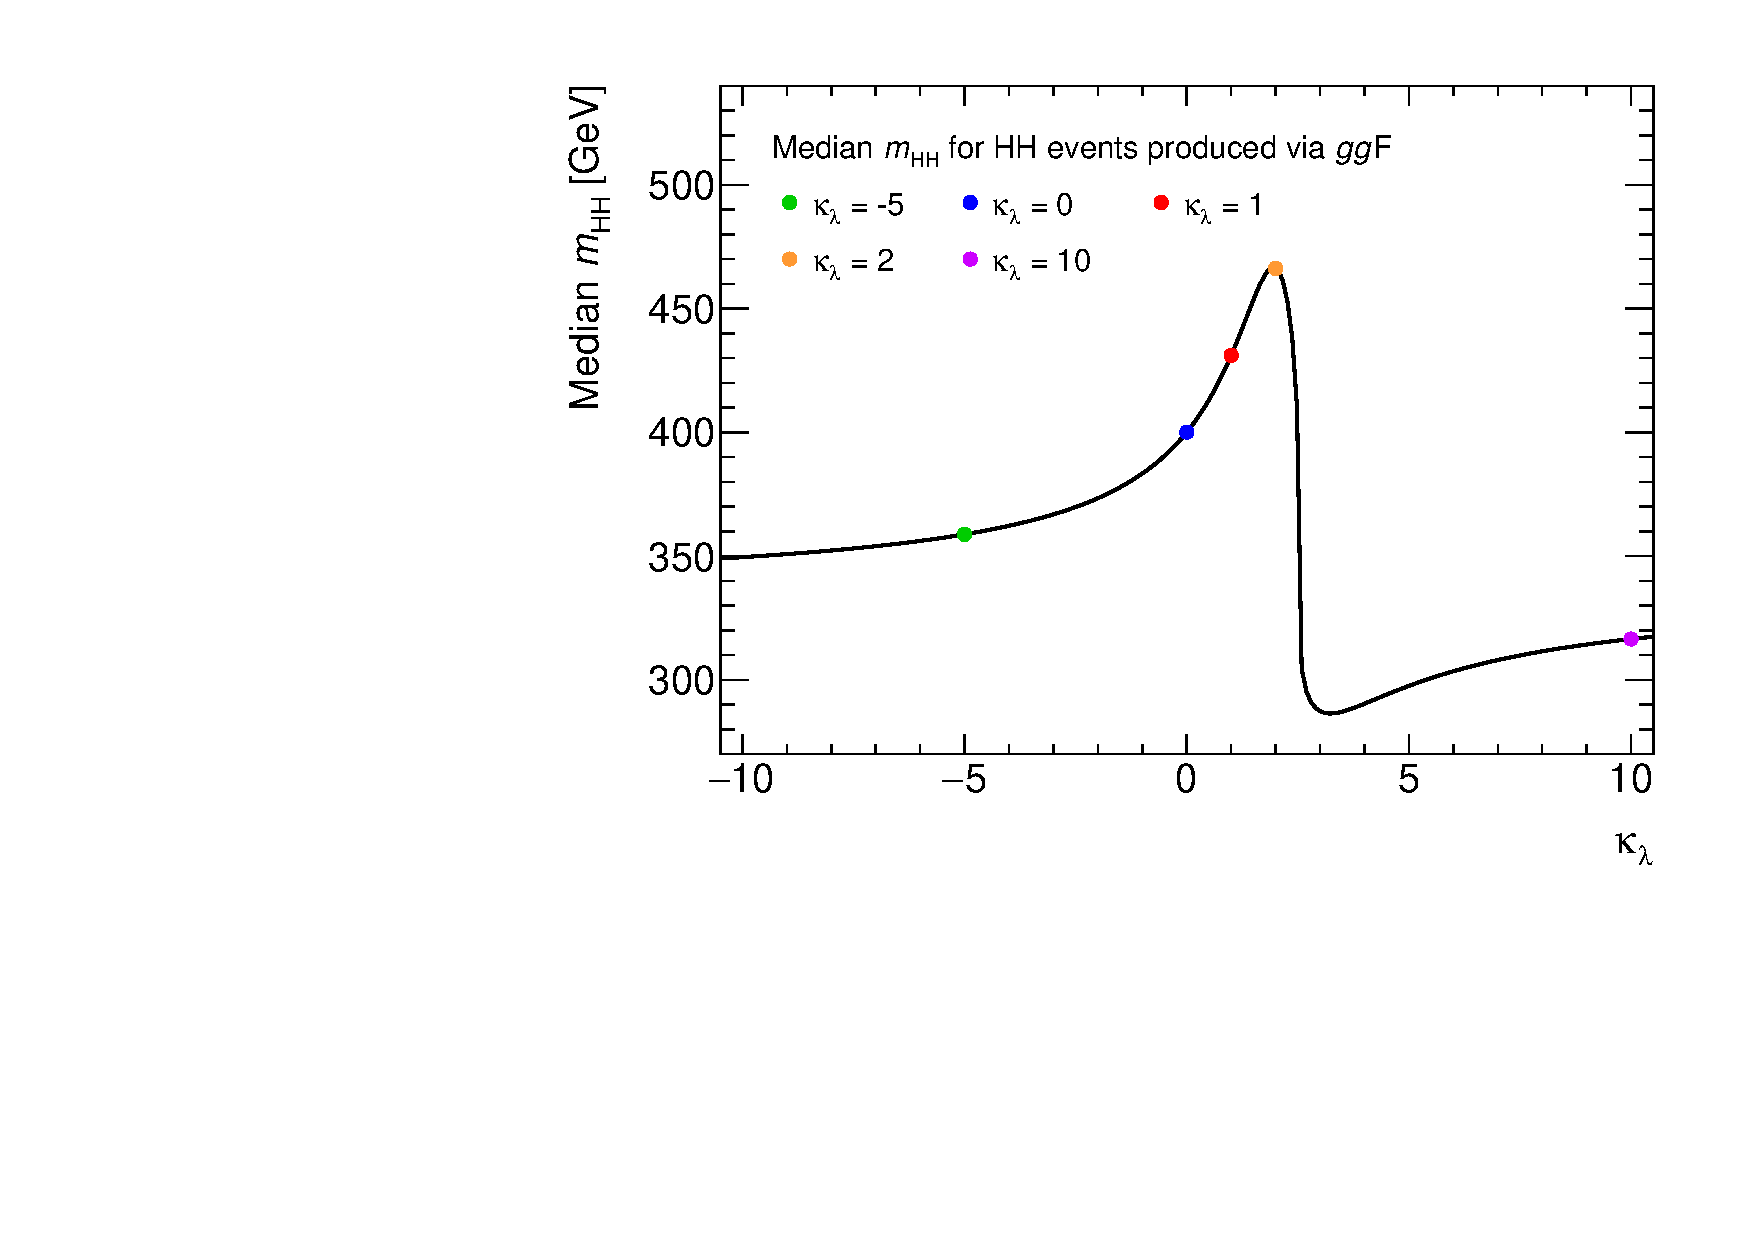
\includegraphics[width=\textwidth]{self_coupling/hh_median_mhh_vs_klam}
    \subcaption{Median value of \mHH for Higgs boson pairs produced
      via \ggF as a function of \klambda.}%
    \label{fig:hh_median_mhh}
  \end{subfigure}

  \caption{Differential cross section of Higgs boson pair production
    via \ggF for selected values of \klambda (a) and the corresponding
    median value of \mHH as a function of \klambda (b). Both are shown
    for \pp-collisions at $\sqrt{s} = \SI{13}{\TeV}$ and assuming
    $\mH= \SI{125.0}{\GeV}$. The cross sections are obtained from
    simulation with \POWHEGBOX[v2] at NLO including the top-quark mass
    dependence~\cite{Heinrich:2019bkc,Heinrich:2020ckp} for
    $\klambda = 0, 1, 10$. Differential cross sections for other
    values of \klambda are estimated using morphing
    techniques~\cite{ATL-PHYS-PUB-2019-007}.}
\end{figure}

This chapter presents a reinterpretation of the search for SM \HH
production ($\klambda = 1$) presented in~\Cref{sec:dihiggs} in terms
of non-resonant \HH production with anomalous values of the Higgs
boson self-coupling constant. A reinterpretation of this search yields
constraints on the allowed values of \klambda as the expected number
of signal events in the signal regions is sensitive to the value of
the self-coupling constant. This sensitivity is due to the \klambda
dependency of both the non-resonant \HH production cross section, and
of the signal acceptance of the selections applied in the analysis
which is closely tied to the characteristic \mHH spectrum of a given
\klambda hypothesis.

Previous constraints on \klambda were set by the ATLAS collaboration
using up to \SI{36.1}{\per\femto\barn} of \pp-collision data taken
during Run~2 of the LHC by combining the results of six searches for
non-resonant \HH production. This combination yielded an allowed range
of $-5.0 < \klambda < 12.0$ at \SI{95}{\percent}
CL~\cite{HDBS-2018-58}. The result presented in this chapter is based
on Ref.~\cite{ATLAS-CONF-2021-052} and focuses on the reinterpretation
of the result obtained in \Cref{sec:dihiggs} in the $\bbbar\tautau$
channel with \SI{139}{\per\femto\barn} of \pp-collision data. The
methodology adopted for the reinterpretation is a continuation of an
earlier result in Ref.~\cite{HDBS-2018-58} by the ATLAS collaboration.

This chapter is structured as follows. \Cref{sec:reinterpretation}
describes the statistical model used for the reinterpretation
including its assumptions and limitations. The resulting constraints
on \klambda are presented in \Cref{sec:reinterpretation_results} and
discussed. The chapter concludes
in~\Cref{sec:reinterpretation_conclusion} with an outlook.


\section{Reinterpretation of the Search for SM \HH Production}%
\label{sec:reinterpretation}

The SM \HH search from \Cref{sec:dihiggs} is reinterpreted to set
upper limits on the cross section of non-resonant \HH production as a
function of the assumed valued of \klambda. These upper limits allow,
by comparison with the theoretical cross section predictions
(cf.~\Cref{fig:hh_xsec_incl}), to exclude regions of \klambda that are
incompatible with the observations made in the SM \HH search. The
reinterpretation adopts the statistical framework presented in
\Cref{sec:statistical_analysis} with few modifications. These
modifications are restricted to the signal model used in the
statistical interpretation. The background model and final
discriminants, including their binning, remain identical to those in
the SM \HH search.

The signal model used for the statistical interpretation is obtained
by replacing the SM \HH ($\klambda = 1$) signal with signals from
non-resonant \HH production with arbitrary but fixed \klambda. Similar
to the SM \HH search, the combination of the \ggF and VBF production
modes is considered as the signal. The cross section of the signal
process, $\sigma_{\text{ggF+VBF}}$, is considered as the parameter of
interest and is allowed to vary freely in the model. The methods for
obtaining signal templates in the signal regions will be described in
\Cref{sec:self_coupling_signals}.

The adopted method of reinterpretation makes assumptions that are
given in the following. First, except for \klambda, all coupling
strengths are assumed to adhere to the SM predictions. Second, the
single Higgs boson production cross sections and branching ratios are
fixed at their SM values and are thus assumed to be independent of
\klambda. This is generally not the case, however, since variations of
\klambda affect both the production cross sections and branching
ratios due to higher-order electroweak corrections. These effects and
their sensitivity to \klambda are discussed in
Refs.~\cite{ATL-PHYS-PUB-2019-009,Degrassi:2016wml,Maltoni:2017ims}.
Since backgrounds from single Higgs boson production are
non-negligible in the SM \HH search, it is instructive to gauge the
crudeness of this approximation over the allowed interval of
$-5.0 < \klambda < 12.0$ from previous results of the ATLAS
collaboration~\cite{HDBS-2018-58}. In the considered \klambda
interval, the single Higgs boson production cross sections deviate
from the SM prediction by up to \SI{12}{\percent} (\SI{25}{\percent})
for the \ggF, VBF, and $VH$ production modes ($\ttbar H$ production
mode)~\cite{ATL-PHYS-PUB-2019-009}. The Higgs boson branching ratios
to fermions show small (relative) deviations of up to \SI{3}{\percent}
from the SM over the relevant \klambda
range~\cite{ATL-PHYS-PUB-2019-009}. For the purpose of this
reinterpretation, signal processes were generated assuming SM Higgs
boson branching ratios for consistency with the treatment of single
Higgs boson backgrounds. A follow-up analysis was performed by the
ATLAS collaboration in Ref.~\cite{ATL-HDBS-2022-03-002} dropping some
of the assumptions made in this chapter.


\subsection{Signal Model for Anomalous Higgs Boson Self-Coupling
  Strengths}%
\label{sec:self_coupling_signals}

Templates of the contribution of a signal with anomalous values of
\klambda in all three signal regions are required to construct the
signal model. These are obtained using morphing and re-weighting
techniques that will be explained hereafter. An ingredient for both
are simulated event samples for different assumed values of
\klambda. The event simulation proceeds using the same generator setup
described previously in \Cref{sec:data_and_simulation}. Non-resonant
\HH events are generated for $\klambda = 1, 10$ for the \ggF
production mode and $\klambda = 0, 1, 10, 20$ for the VBF production
mode. Additionally, large samples of events from non-resonant \HH
production via \ggF are generated for $\klambda = 0, 1, 10, 20$
without simulation of the ATLAS detector. These event samples are
normalised using the cross sections previously shown in
\Cref{fig:hh_xsec_incl}.

% Based on: (?)
% https://link.springer.com/content/pdf/10.1007/JHEP06(2019)066.pdf
At LO in \klambda the amplitudes involved in Higgs boson pair
production can be written as $\klambda \mathcal{A} + \mathcal{B}$
where $\mathcal{A}$ is the amplitude of diagrams involving the Higgs
boson self-coupling and $\mathcal{B}$ summarises all other
contributing diagrams. Squaring the amplitude results in a term from
the diagram involving the Higgs boson self-coupling proportional to
$\klambda^2$, an interference term proportional to $\klambda$, and the
term originating from diagrams without Higgs boson
self-coupling. These considerations are applicable both to the \ggF
and the VBF production modes.

- Re-weighting

- Uncertainties


ggF: Re-weighting

VBF: Linear combination

\todo[inline]{Hadhad channel: Acceptance times efficiency vs mHH.}

\todo[inline]{Hadhad channel: Acceptance times efficiency vs kLambda.}

Should say that bbtautau is only good because the SM is already pretty
hard. -> acceptance vs mHH in \hadhad.


Signal modelling uncertainties:
- Uncertainties from the re-weighting procedure are included
- The signal modelling uncertainties are included

\begin{figure}[htbp]
  \centering

  \begin{subfigure}[t]{0.485\textwidth}
    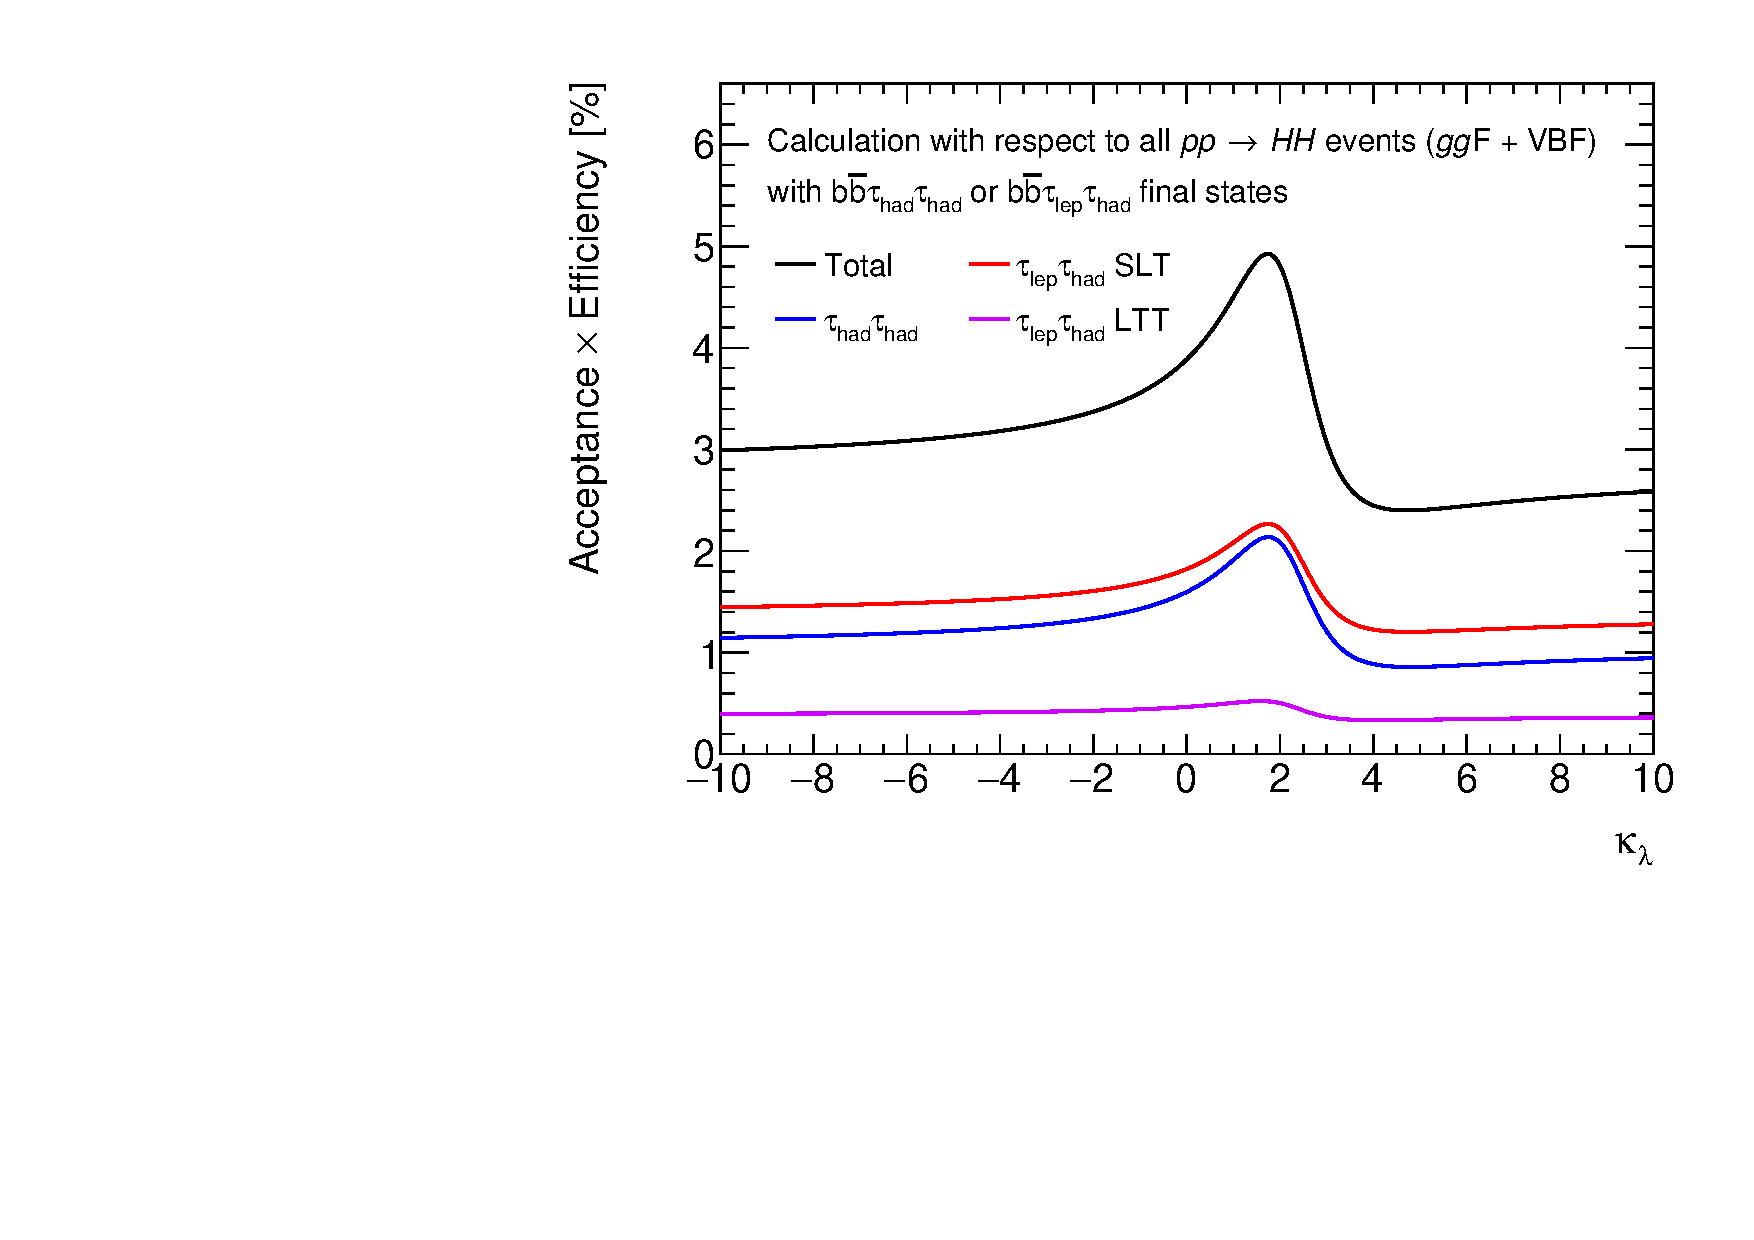
\includegraphics[width=\textwidth]{self_coupling/acc_vs_klam}
    \subcaption{}
  \end{subfigure}\hfill%
  \begin{subfigure}[t]{0.485\textwidth}
    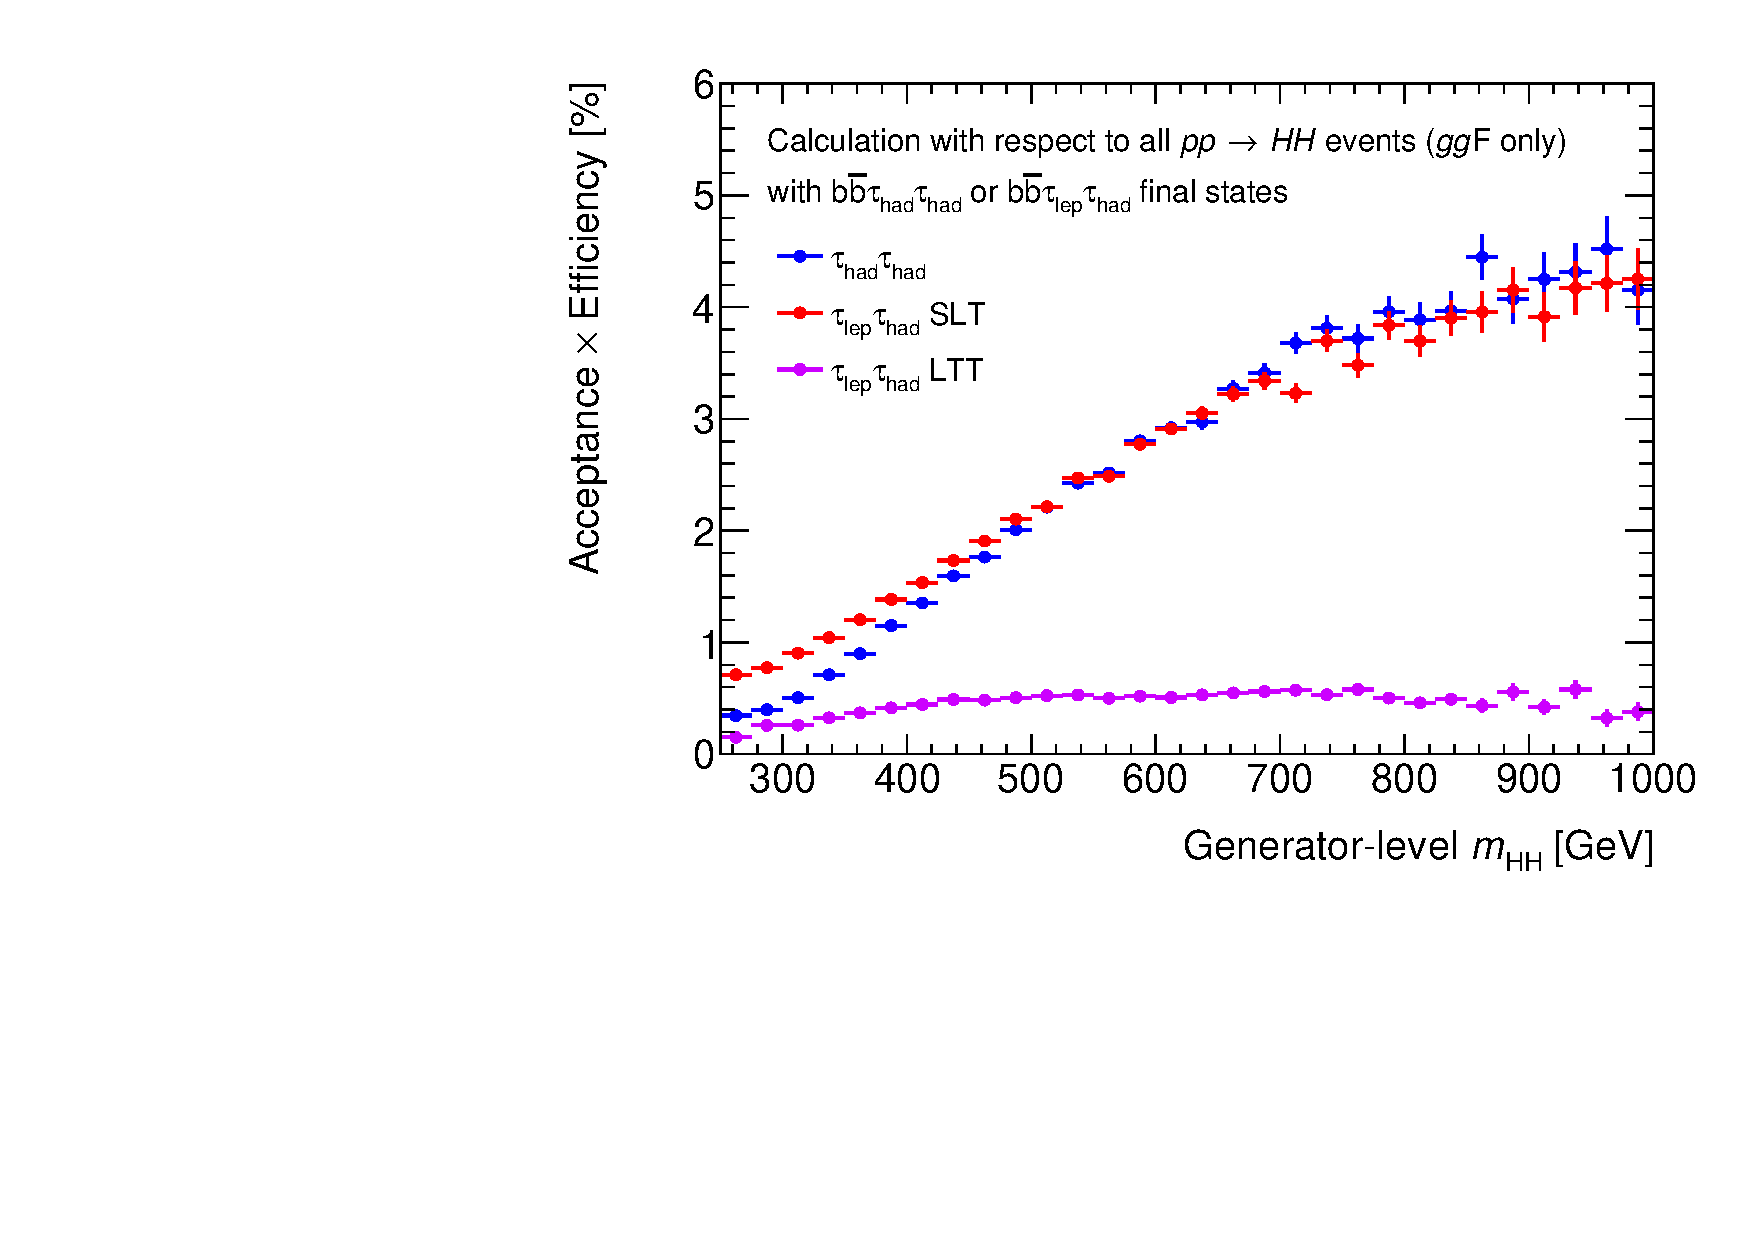
\includegraphics[width=\textwidth]{self_coupling/acc_vs_mhh}
    \subcaption{}
  \end{subfigure}

  \caption{}%
  \label{fig:acceptance_vs_klambda}
\end{figure}


\section{Results}%
\label{sec:reinterpretation_results}


\begin{figure}[htbp]
  \centering

  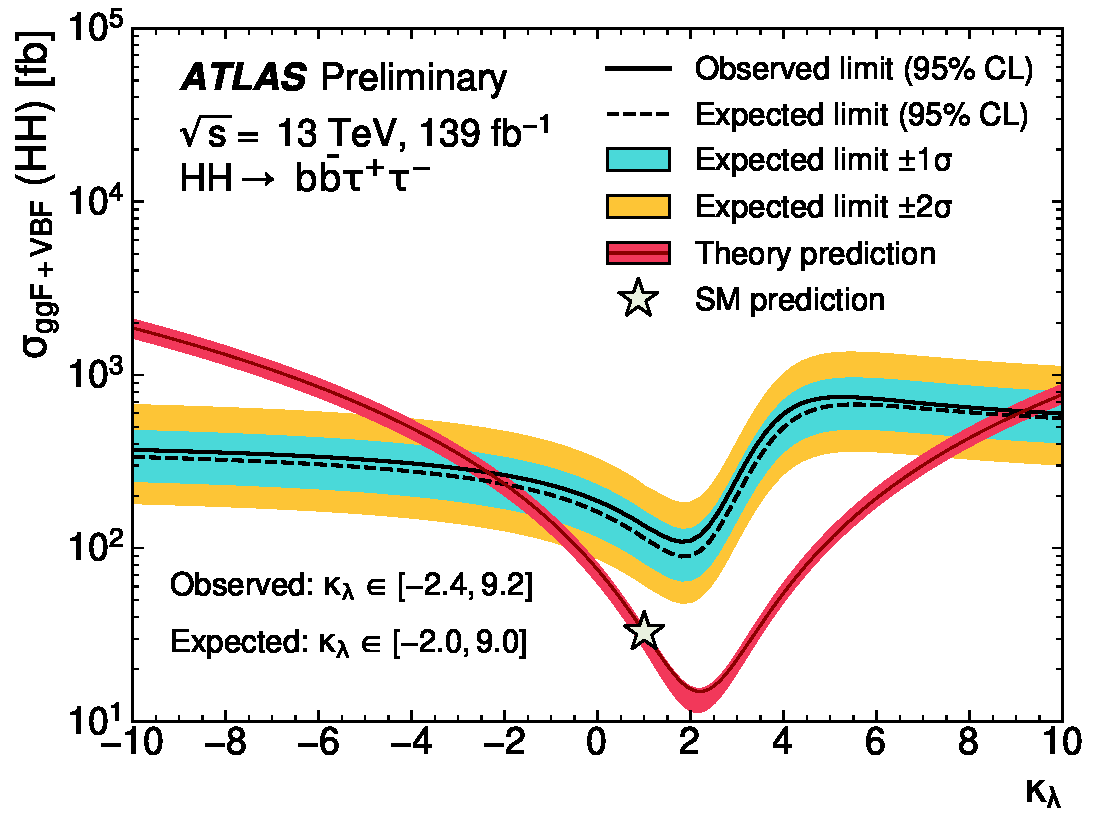
\includegraphics[width=0.6\textwidth]{self_coupling/klam_scan_result}

  \caption{Klambda scan. The figure is taken from
    Ref.~\cite{ATLAS-CONF-2021-052}.}%
  \label{fig:klambda_scan}
\end{figure}

Upper limits are set on $\sigma_{HH}^{\klambda}$ as a function of
\klambda and compare to the theoretical cross section for a given
value of \klambda. Intervals of \klambda are excluded if the cross
section predicted by theory is larger than the experimentally
determined upper limit.


\section{Conclusion and Outlook}%
\label{sec:reinterpretation_conclusion}


The total Higgs boson pair production cross section with anomalous
couplings. Following recommendations by the LHC Higgs Working
Group~\cite{LHCHWGHH}:
\begin{description}

\item[\ggF production mode] The cross sections of \HH production with
  anomalous self-couplings were calculated in
  Ref.~\cite{Amoroso:2020lgh} at $\text{NNLO}_{\text{NLO-i}}$
  (NLO-improved). This prediction is obtained from combining the
  result with the full top-quark mass dependence at
  NLO~\cite{Buchalla:2018yce}


  with NNLO corrections in the $m_{t} \to \infty$
  limit~\cite{deFlorian:2017qfk}.

  Additionally, the prediction is rescaled such that it coincides with
  the SM \HH cross section at $\text{NNLO}_{\text{FTapprox}}$ at
  $\klambda = 1$.

  The total \HH production cross section via \ggF was found to depend
  quadratically on \klambda and is thus parameterised
  accordingly~\cite{LHCHWGHH}.

\item[VBF production mode]

\end{description}


\todo[inline]{Read YR about Higgs cross section predictions:
  \url{https://cds.cern.ch/record/2227475/files/CERN-2017-002-M.pdf}}

Sample combination method:~\cite{ATL-PHYS-PUB-2019-007}


\todo{Updated result from H+HH
  combination~\cite{ATLAS-CONF-2022-050}.}

These results were superseded by a combination of the most sensitive
search channels for non-resonant \HH and single Higgs boson production
by the ATLAS collaboration in Ref.~\cite{ATLAS-CONF-2022-050}, which
is not discussed in detail in this chapter.


%%% Local Variables:
%%% mode: latex
%%% TeX-master: "../../phd_thesis"
%%% End:
